\chapter{Ownership Transfer}
\label{sec:hla-own}

There are two \TrickHLA\ mechanisms for initiating ownership transfer:
the current owner may {\em divest} itself of ownership contingent on the
existence of some other federate that is willing to assume it,
or a non-owner may {\em acquire} ownership from the current owner
contingent on that federate being willing.
The \TrickHLA\ terminology for these two approaches to ownership  transfer
is {\em push} and {\em pull}, respectively.
This chapter illustrates how to write simulations that push and/or pull
ownership.

The simulations we present are
\begin{itemize}
\item{
  A publisher that initially owns the \simplesine state
  and {\em pushes} ownership away at a specified time in the run
  then at some subsequent time {\em pulls} ownership back, and
}
\item{
  Another publisher that does not initially own the \simplesine state
  but will assume ownership when the other federate divests it and will
  surrender it when the original federate tries to pull ownership back.
}
\end{itemize}

\TrickHLA\ automatically ensures that publishers
(federates who explicitly indicate their {\em ability}
to update the associated data)
are eligible to assume ownership when the current owner divests
itself of ownership by invoking the \TrickHLA\ {\em push} method.
The non-owning publisher does not need to take any explicit action
for this to happen.\footnote{
  Thus, in the HLA nomenclature, the distinction between a
  publisher that {\em owns} the object/attributes and a
  publisher that {\em does not own} them is important.
  For former may generate updates for them, and the latter may not.
  Thus, ownership tranfer leads to a change in which publisher
  is actually generating data updates.
}
Similarly, when a non-owning publisher invokes the
\TrickHLA\ {\em pull} method, transfer of ownership from the current owner
to the requesting federate is automatically handled.
The current owner needs not explicitly handle the transfer request.\footnote{
  Indeed, \TrickHLA\ does not currently provide any mechanism
  for the current owner to decline a pull request.
}

% ---------------------------------------------------------------------
\section{What is an ownership handler?}

\TrickHLA\ includes a utility class that may be used directly
(i.e., no subclassing necessary)
to push and pull ownership.
The class header is shown below.

\begin{lstlisting}[caption={{\tt TrickHLAOwnershipHandler} class header}]
#include <string>

#include "TrickHLA/include/TrickHLAStandardsSupport.hh"
class TrickHLAObject;
class TrickHLAAttribute;
#include "TrickHLA/include/TrickHLAObject.hh"
#include "TrickHLA/include/TrickHLAAttribute.hh"
#include "TrickHLA/include/TrickHLATypesNoICG.hh"
#include "TrickHLA/include/TrickHLAOwnershipHandlerNoICG.hh"
#include "TrickHLA/include/TrickHLAOwnershipItem.hh"
#include "TrickHLA/include/TrickHLADoubleInterval.hh"
#include "TrickHLA/include/TrickHLADoubleTime.hh"

#include RTI1516_HEADER

using namespace std;
using namespace RTI1516_NAMESPACE;

class TrickHLAOwnershipHandler
{
  friend class InputProcessor;
  friend void init_attrTrickHLAOwnershipHandler();

  friend class TrickHLAObject;
  
  public:
   TrickHLAOwnershipHandler();
   virtual ~TrickHLAOwnershipHandler();

   void checkpoint_requests();
   void clear_checkpoint();
   void restore_requests();
   
   virtual void initialize_callback( TrickHLAObject * obj );

   string get_object_name();
   string get_object_FOM_name();

   int get_attribute_count();
   VectorOfStrings get_attribute_FOM_names() const;

   bool is_locally_owned( const char * attribute_FOM_name );
   bool is_remotely_owned( const char * attribute_FOM_name );

   bool is_published( const char * attribute_FOM_name );
   bool is_subscribed( const char * attribute_FOM_name );

   void pull_ownership();
   void pull_ownership( double time );
   void pull_ownership( const char * attribute_FOM_name );
   void pull_ownership( const char * attribute_FOM_name, double time );

   void push_ownership();
   void push_ownership( double time );
   void push_ownership( const char * attribute_FOM_name );
   void push_ownership( const char * attribute_FOM_name, double time );

   TrickHLADoubleInterval get_fed_lookahead();
   TrickHLADoubleTime     get_granted_fed_time();

  private:
   TrickHLAAttribute * get_attribute( const char * attribute_FOM_name );
   TrickHLAObject * object;    // ** Reference to the TrickHLA Object.
   AttributeOwnershipMap pull_requests; // ** Map of pull ownership user requests.
   AttributeOwnershipMap push_requests; // ** Map of push ownership user requests.
   int                     pull_items_cnt; // -- # of pull items
   TrickHLAOwnershipItem * pull_items;     // -- array of pulled attributes
   int                     push_items_cnt; // -- # of push items
   TrickHLAOwnershipItem * push_items;     // -- array of pushed attributes
};
\end{lstlisting}

The {\tt pull\_ownership()} and {\tt push\_ownership()} methods are of
particular interest.
The methods without arguments push or pull all the attributes of the
associated object immediately.
The methods with only a time argument push or pull all the attributes of the
specific object at the specified future time.
And the methods with an explicit attribute name argument allow pushing and
pulling of single attributes within an object without affecting the others.

% ---------------------------------------------------------------------
\section{\tt SIM\_simplesine\_hla\_own}

Our illustration of how to use the {\tt TrickHLAOwnershipHandler} class
involves two different instances of a single simulation.

The first instance is the {\em active} publisher that
initially owns the relevant object and attributes
and explicitly calls the {\tt push\_ownership()} and {\tt pull\_ownership()}
methods.
The second instance is a {\em passive} publisher that does not initially
own the object and attributes, nor does it explicitly request any ownership
transfers.
Instead, the passive instance of the simulation gains and surrenders
ownership as the result of the remote push/pull requests by the active
instance.

Both instances not only publish the \simplesine data, but they also
subscribe, allowing them to receive updates from the other instance
when the object and attributes are remotely owned.

The two instances share the same \sdefine file, which is derived from
the plain publisher.
The only differences between the \sdefine file for the
{\tt SIM\_simplesine\_hla\_own} simulation
and that of the plain publisher are

\begin{itemize}
\item{
  an ownership handler variable is defined by adding the following line,
  \begin{verbatim}
 TrickHLA: TrickHLAOwnershipHandler ownership_handler; \end{verbatim}
}
\item{
  and zero-frequency jobs are declared for
  {\tt push\_ownership()} and {\tt pull\_ownership()}
  as follows
  \begin{verbatim}
 (0.0, scheduled) TrickHLA: publisher.ownership_handler.push_ownership();
 (0.0, scheduled) TrickHLA: publisher.ownership_handler.pull_ownership(); \end{verbatim}
  so that the methods may be invoked from the input file using the
  {\tt CALL} directive.
}
\end{itemize}

% ---------------------------------------------------------------------
\section{Active input file}

The input file for the active ownership transfer simulation is
based on the input file for the plain publisher.
The differences are:

\begin{itemize}
\item{
  A new file, {\tt LogData/THLA\_objects.d} is included.
  This file contains inputs that ensure that the ownership flag
  {\tt THLA.manager.objects[0].attributes[0].locally\_owned} is logged.
  This allows us to plot the ownership transfer as it takes place.
}
\item{
  The federate name is {\em active} instead of {\em publisher}.
}
\item{
  The federate waits for a second federate named {\em passive}
  instead of {\em subscriber}.
}
\item{
  The ownership handler defined in the \sdefine file is associated
  with the object as follows.
  \begin{verbatim}
  THLA.manager.objects[0].ownership = &publisher.ownership_handler; \end{verbatim}
}
\item{
  The {\tt .subscribe} flag of the object's attributes are all set to
  true so that the simulation will receive updated values when the
  other federate owns the object.
}
\item{
  The simulation {\em pushes} ownership away at $t=5$ using the {\tt CALL}
  directive as follows.
  \begin{verbatim}
 read = 5.0;
 CALL publisher.publisher.ownership_handler.push_ownership(); \end{verbatim}
}
\item{
  And finally the simulation {\em pulls} ownership back at $t=10$
  as follows.
  \begin{verbatim}
 read = 10.0;
 CALL publisher.publisher.ownership_handler.pull_ownership(); \end{verbatim}
}
\end{itemize}

% ---------------------------------------------------------------------
\section{Passive input file}

The input file for the passive ownership transfer simulation is
virtually identical to the active input file with the following exceptions.

\begin{itemize}
\item{
  The federate name is {\em passive}.
}
\item{
  The attribute {\tt .locally\_owned} flags are initially false,
  since at simulation start the passive simulation does not own them.
}
\item{
  There are no {\tt CALL} directives.
}
\end{itemize}

That last point deserves emphasizing.
This simulation accepts ownership when the {\em active} federate pushes
ownership away from itself; no explicit action is required on the part
of the passive simulation in order to accept ownerhip.
Similarly,
this simulation willingly surrenders ownership when the {\em active}
federate pulls it back; again, this happens without any explicit action
on the part of the passive simulation.

% ---------------------------------------------------------------------
\section{Output}

Inspection of the (abbreviated) output shown below from the active simulation
reveals that it does indeed divest ownership and then reacquire it later.

\begin{lstlisting}[numbers=none,caption={Output stream from the active ownerhsip transfer simulation}]
...
| |wormhole|1|3.00|2007/08/05,21:56:18| TrickHLAManager::receive_cyclic_data()
| |wormhole|1|3.00|2007/08/05,21:56:18| TrickHLAManager::send_cyclic_data()
| |wormhole|-1|3.25|2007/08/05,21:56:18| TrickHLAFedAmb::timeAdvanceGrant()
Federate "active" Time granted to: 4
| |wormhole|1|4.00|2007/08/05,21:56:19| TrickHLAManager::receive_cyclic_data()
| |wormhole|1|4.00|2007/08/05,21:56:19| TrickHLAManager::send_cyclic_data()
| |wormhole|-1|4.25|2007/08/05,21:56:19| TrickHLAFedAmb::timeAdvanceGrant()
Federate "active" Time granted to: 5
| |wormhole|1|5.00|2007/08/05,21:56:20| TrickHLAManager::receive_cyclic_data()
| |wormhole|1|5.00|2007/08/05,21:56:20| TrickHLAManager::send_cyclic_data()
| |wormhole|1|5.00|2007/08/05,21:56:20| TrickHLAObject::push_ownership()
...
| |wormhole|1|6.00|2007/08/05,21:56:21| TrickHLAObject::release_ownership()
   DIVESTED Ownership of attribute 'SimplesineStateAndParameters'->'Time'
   of object 'simplesineStateAndParameters'.
| |wormhole|1|6.00|2007/08/05,21:56:21| TrickHLAObject::release_ownership()
   DIVESTED Ownership of attribute 'SimplesineStateAndParameters'->'Value'
   of object 'simplesineStateAndParameters'.
| |wormhole|1|6.00|2007/08/05,21:56:21| TrickHLAObject::release_ownership()
   DIVESTED Ownership of attribute 'SimplesineStateAndParameters'->'dvdt'
   of object 'simplesineStateAndParameters'.
| |wormhole|1|6.00|2007/08/05,21:56:21| TrickHLAObject::release_ownership()
   DIVESTED Ownership of attribute 'SimplesineStateAndParameters'->'Phase'
   of object 'simplesineStateAndParameters'.
| |wormhole|1|6.00|2007/08/05,21:56:21| TrickHLAObject::release_ownership()
   DIVESTED Ownership of attribute 'SimplesineStateAndParameters'->'Frequency'
   of object 'simplesineStateAndParameters'.
| |wormhole|1|6.00|2007/08/05,21:56:21| TrickHLAObject::release_ownership()
   DIVESTED Ownership of attribute 'SimplesineStateAndParameters'->'Amplitude'
   of object 'simplesineStateAndParameters'.
...
| |wormhole|1|9.00|2007/08/05,21:56:24| TrickHLAManager::receive_cyclic_data()
| |wormhole|1|9.00|2007/08/05,21:56:24| TrickHLAManager::send_cyclic_data()
| |wormhole|-1|9.25|2007/08/05,21:56:24| TrickHLAFedAmb::timeAdvanceGrant()
Federate "active" Time granted to: 10
| |wormhole|1|10.00|2007/08/05,21:56:25| TrickHLAManager::receive_cyclic_data()
| |wormhole|1|10.00|2007/08/05,21:56:25| TrickHLAManager::send_cyclic_data()
| |wormhole|1|10.00|2007/08/05,21:56:25| TrickHLAObject::pull_ownership()
...
   ACQUIRED ownership of attribute 'SimplesineStateAndParameters'->'Time'
   of object 'simplesineStateAndParameters'.
| |wormhole|-1|11.25|2007/08/05,21:56:26| TrickHLAFedAmb::attributeOwnershipAcquisitionNotification()
   ACQUIRED ownership of attribute 'SimplesineStateAndParameters'->'Value'
   of object 'simplesineStateAndParameters'.
| |wormhole|-1|11.25|2007/08/05,21:56:26| TrickHLAFedAmb::attributeOwnershipAcquisitionNotification()
   ACQUIRED ownership of attribute 'SimplesineStateAndParameters'->'dvdt'
   of object 'simplesineStateAndParameters'.
| |wormhole|-1|11.25|2007/08/05,21:56:26| TrickHLAFedAmb::attributeOwnershipAcquisitionNotification()
   ACQUIRED ownership of attribute 'SimplesineStateAndParameters'->'Phase'
   of object 'simplesineStateAndParameters'.
| |wormhole|-1|11.25|2007/08/05,21:56:26| TrickHLAFedAmb::attributeOwnershipAcquisitionNotification()
   ACQUIRED ownership of attribute 'SimplesineStateAndParameters'->'Frequency'
   of object 'simplesineStateAndParameters'.
| |wormhole|-1|11.25|2007/08/05,21:56:26| TrickHLAFedAmb::attributeOwnershipAcquisitionNotification()
   ACQUIRED ownership of attribute 'SimplesineStateAndParameters'->'Amplitude'
   of object 'simplesineStateAndParameters'.
...
\end{lstlisting}

On the other side,
inspection of the (abbreviated) output shown below from the passive simulation
reveals that it does indeed acquire ownership and then divest it later.

\begin{lstlisting}[numbers=none,caption={Output stream from the passive ownerhsip transfer simulation}]
...
| |wormhole|1|4.00|2007/08/05,21:56:19| TrickHLAManager::receive_cyclic_data()
| |wormhole|1|4.00|2007/08/05,21:56:19| TrickHLAManager::send_cyclic_data()
| |wormhole|-1|4.25|2007/08/05,21:56:19| TrickHLAFedAmb::timeAdvanceGrant()
Federate "passive" Time granted to: 5
| |wormhole|1|5.00|2007/08/05,21:56:20| TrickHLAManager::receive_cyclic_data()
| |wormhole|1|5.00|2007/08/05,21:56:20| TrickHLAManager::send_cyclic_data()
| |wormhole|-1|5.25|2007/08/05,21:56:20| TrickHLAFedAmb::timeAdvanceGrant()
Federate "passive" Time granted to: 6
| |wormhole|-1|5.25|2007/08/05,21:56:20| TrickHLAFedAmb::requestAttributeOwnershipAssumption()
  push request received, tag='simplesineStateAndParameters'
| |wormhole|-1|5.25|2007/08/05,21:56:20| TrickHLAFedAmb::requestAttributeOwnershipAssumption()
...
| |wormhole|-1|6.25|2007/08/05,21:56:21| TrickHLAFedAmb::attributeOwnershipAcquisitionNotification()
   ACQUIRED ownership of attribute 'SimplesineStateAndParameters'->'Time'
   of object 'simplesineStateAndParameters'.
| |wormhole|-1|6.25|2007/08/05,21:56:21| TrickHLAFedAmb::attributeOwnershipAcquisitionNotification()
   ACQUIRED ownership of attribute 'SimplesineStateAndParameters'->'Value'
   of object 'simplesineStateAndParameters'.
| |wormhole|-1|6.25|2007/08/05,21:56:21| TrickHLAFedAmb::attributeOwnershipAcquisitionNotification()
   ACQUIRED ownership of attribute 'SimplesineStateAndParameters'->'dvdt'
   of object 'simplesineStateAndParameters'.
| |wormhole|-1|6.25|2007/08/05,21:56:21| TrickHLAFedAmb::attributeOwnershipAcquisitionNotification()
   ACQUIRED ownership of attribute 'SimplesineStateAndParameters'->'Phase'
   of object 'simplesineStateAndParameters'.
| |wormhole|-1|6.25|2007/08/05,21:56:21| TrickHLAFedAmb::attributeOwnershipAcquisitionNotification()
   ACQUIRED ownership of attribute 'SimplesineStateAndParameters'->'Frequency'
   of object 'simplesineStateAndParameters'.
| |wormhole|-1|6.25|2007/08/05,21:56:21| TrickHLAFedAmb::attributeOwnershipAcquisitionNotification()
   ACQUIRED ownership of attribute 'SimplesineStateAndParameters'->'Amplitude'
   of object 'simplesineStateAndParameters'.
| |wormhole|-1|6.25|2007/08/05,21:56:21| TrickHLAFedAmb::timeAdvanceGrant()
Federate "passive" Time granted to: 7
...
| |wormhole|-1|10.25|2007/08/05,21:56:25| TrickHLAFedAmb::requestAttributeOwnershipRelease()
  pull request received, tag='simplesineStateAndParameters'
| |wormhole|-1|10.25|2007/08/05,21:56:25| TrickHLAFedAmb::requestAttributeOwnershipRelease()
...
   DIVESTED Ownership for attribute 'SimplesineStateAndParameters'->'Time'
   of object 'simplesineStateAndParameters'.
| |wormhole|1|11.00|2007/08/05,21:56:26| TrickHLAObject::grant_pull_request()
   DIVESTED Ownership for attribute 'SimplesineStateAndParameters'->'Value'
   of object 'simplesineStateAndParameters'.
| |wormhole|1|11.00|2007/08/05,21:56:26| TrickHLAObject::grant_pull_request()
   DIVESTED Ownership for attribute 'SimplesineStateAndParameters'->'dvdt'
   of object 'simplesineStateAndParameters'.
| |wormhole|1|11.00|2007/08/05,21:56:26| TrickHLAObject::grant_pull_request()
   DIVESTED Ownership for attribute 'SimplesineStateAndParameters'->'Phase'
   of object 'simplesineStateAndParameters'.
| |wormhole|1|11.00|2007/08/05,21:56:26| TrickHLAObject::grant_pull_request()
   DIVESTED Ownership for attribute 'SimplesineStateAndParameters'->'Frequency'
   of object 'simplesineStateAndParameters'.
| |wormhole|1|11.00|2007/08/05,21:56:26| TrickHLAObject::grant_pull_request()
   DIVESTED Ownership for attribute 'SimplesineStateAndParameters'->'Amplitude'
   of object 'simplesineStateAndParameters'.
...
\end{lstlisting}

This is also illustrated in the two following plots of the
{\tt .locally\_owned} flag for the first attribute of the object.

\clearpage

\begin{figure}[h]
  \begin{center}
    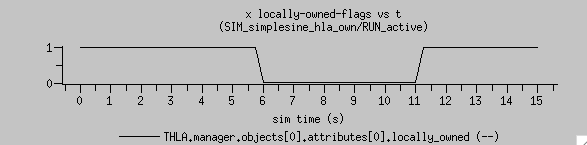
\includegraphics[width=5.5in]{TrickHLAUser-SIM-hla-own-active.png}
  \end{center}
\caption{Output from the active {\tt SIM\_simplesine\_hla\_own} simulation}
\label{fig:hla-own-active-output}
\end{figure}


\begin{figure}[h]
  \begin{center}
    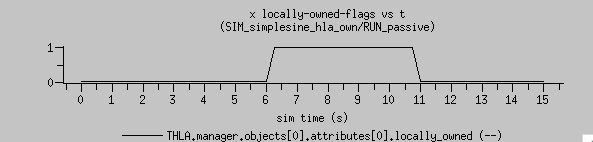
\includegraphics[width=5.5in]{TrickHLAUser-SIM-hla-own-passive.png}
  \end{center}
\caption{Output from the passive {\tt SIM\_simplesine\_hla\_own} simulation}
\label{fig:hla-own-passive-output}
\end{figure}

\clearpage
